\section{Meccanica Lagrangiana}


\subsection{Sistemi potenziali newtoniani}

Consideriamo il sistema newtoniano costruito da $n $ particelle di masse $m_1,m_2,\dots,m_n$, interagenti tramite forze potenziali.\\
Precisamente supponiamo esista un potenziale:
\begin{equation}
    U(x^{(1)}, \dots, x^{(n )},t) \quad \text{ con } x^{(i )}\in \mathbb{R}^d  
\end{equation}
dove $x^{(i )}$ è la posizione della $i $-esima particella.\\
Tale che:
\begin{equation}
    f^{(i)}:= -\nabla_{(x^{(i)})}U= -\pdv{U}{x^{(i)}}= -\begin{pmatrix}
        \partial_{x^{(i)}_1}U\\
        \vdots\\
        \partial_{x^{(i)}_d}U
    \end{pmatrix}
\end{equation}
Il sistema di equazioni di Newton diventa:
\begin{equation}
    m_i\ddot{x}^{(i)}= f^{(i)}= -\pdv{U}{x^{(i)}}\iff\begin{cases}
        m_1\ddot{x}^{(1)}= \pdv{U}{x^{(1)}}\\
        \vdots\\
        m_n \ddot{x}^{(n)}= \pdv{U}{x^{(n)}}
    \end{cases}
\end{equation}
\begin{theorem}
    \begin{equation*}
        \pdv{U}{t}=0\implies H = \sum_{i=1}^{n}\frac{m_i}{2}\abs{\dot{x}^{(i)}}^2 + U (x^{(1)},\dots,x^{(n)}) \text{  si conserva.}
    \end{equation*}
\end{theorem}
\begin{proof}
    \begin{equation*}
        \dv{H}{t}= \sum_{i=1}^{n} m_i \dot{x}^{(i)}\cdot\ddot{x}^{(i)}+ \sum_{i=1}^{n}\pdv{U}{x^{(i)}}\cdot \dot{x}^{(i)}
    \end{equation*}
    \begin{equation*}
        = \sum_{i=1}^{n} \dot{x}^{(i)}\left( m_i\ddot{x}^{(i)}+\pdv{U}{x^{(i)}} \right)=0
    \end{equation*}
\end{proof}

Per comodità definifiamo:
\begin{equation}
    X:=\begin{pmatrix}
        x^{(1)}\\\vdots\\x^{(n )}
    \end{pmatrix}
    \in \mathbb{R}^d \times \dots \times \mathbb{R}^d \simeq \mathbb{R}^{nd}\qquad N = nd
\end{equation}
\begin{equation}
    \implies M\ddot{X}= -\nabla_X U\,; \qquad f = -\nabla_X U = \left( \pdv{U}{x^{(1)}};\dots;\pdv{U}{x^{(n)}} \right)\in \mathbb{R}^N 
\end{equation}
Dove la \textit{matrice delle masse }$M = \operatorname{diag} (m_1 \mathds{1}_d, \dots, m_n\mathds{1}_d)$ .
\begin{equation}
     M\ddot{X}= -\pdv{U}{X}\iff
    \begin{cases}
        \dot{X}= V\\\dot{V}= - M^{-1}\nabla_X U
    \end{cases}
\end{equation}
$X \in \mathbb{R}^N$ si dice \textit{spazio delle configurazioni del sistema}.\\
$(X,V)\in \mathbb{R}^N \times \mathbb{R}^N \simeq \mathbb{R}^{2N}$ si dice \textit{spazio delle fasi del sistema}.

\begin{samepage}
Affronteremo due problemi:
\begin{itemize}
    \item Come studiare il sistema in casi di dinamica vincolata:\begin{equation*}
        \begin{cases}
            M\ddot{X}= -\nabla_X U\\ X \in \mathcal{M}
        \end{cases}
        \end{equation*}
        dove $\mathcal{M}$ è una varietà differenziabile.
    \item Come varia il sistema sottoposto a un cambio di coordinate:\begin{equation*}
        \begin{cases}
            M\ddot{X} = -\nabla_X U\\ X \rightarrow X'
        \end{cases}
    \end{equation*}
\end{itemize}
\end{samepage}

\paragraph{Vincoli}
Esistono diversi tipi di vincoli:
\begin{itemize}
    \item \textbf{Vincolo bilatero:} vincola la particella a muoversi su una determinata curva o superficie.
    \item \textbf{Vincolo unilatero: } vincola la particella a non attraversare il determinato vincolo.
\end{itemize}
Noi ci limiteremo a studiare i vincoli bilateri e posizionali (\textit{olonomi}), che coinvolgono solo la posizione e non le velocità.

\begin{example}
    \textbf{Cerchio di raggio $r$}
    \begin{equation*}
        f(x_1,x_2)= x_1^2+x_2^2-r=0
    \end{equation*}
\end{example}

%fare meglio esempio e aggiunugere sfera e paraboloide


\subsection{Varietà differenziali}

\begin{definition}
    Data una funzione $\Phi: \mathbb{R}^N \times \mathbb{R}\rightarrow \mathbb{R}^M:(X,t)\mapsto \Phi(X,t)$ di classe $\mathcal{C}^1$,
    l'insieme di livello $\Phi^{-1}(0)= \left\{ X\in \mathbb{R}^N \;t.c.\; \Phi(x,t)=0\right\}$ definisce una \textit{varietà differenziabile}
    di classe $\mathcal{C}^1$ e dimensione $L=N-M $ se 
    \begin{equation}
        \pdv{\Phi}{X}= \pdv{\left( \Phi_1,\dots,\Phi_M \right)}{\left( X_1,\dots, X_N \right)}
    \end{equation} ha rango massimo $M $.
\end{definition}
\begin{theorem}
    Data $\Phi^{-1}(0) $ varietà differenziabile, esiste sempre \textit{rappresentazione cartesiana locale} per almeno un set di $L $ cooridnate libere:
    \begin{equation}
        \begin{cases}
            X_1 = g_1(X_{M+1},\dots,X_N)\\\vdots\\X_M = g_M (X_{M+1},\dots, X_N )
        \end{cases}
    \end{equation}
    Inoltre esiste una \textit{rappresentazione parametrica}.
\end{theorem}
\begin{proof}
    La prima parte si dimostra con il teorema di Dini, la seconda è ovvia. Riscriviamo le \( X_{M+1}, \dots, X_N \) come funzione di parametri liberi (cambio di coordinate) \( X_{M+i} = h_i(n_1, \dots, n_L) \) (può bastare \( X_{M+i} = n_i \)), e poi:
    \begin{equation*}
        \begin{cases}
            X_1 = g_1(f_1(n), \dots, f_L(n), t) := h_1(n, t)\\
            \vdots\\
            X_M = g_M(f_1(n), \dots, f_L(n), t) := h_M(n, t)\\
            X_{M+1} = f_1(n) := h_{M+1}(n, t)\\
            \vdots\\
            X_N = f_L(n) := h_N(n, t)
        \end{cases}
    \end{equation*}
    In conclusione, possiamo pensare alla varietà \(\mathcal{M}_t\) come localmente definita in forma parametrica \( \mathbb{R}^L \ni \vec{n} \mapsto X(\vec{n}, t) \in \mathbb{R}^N \), con dipendenza esplicita dal tempo.
\end{proof}

\begin{definition}
    $M= N-L $ si dice \textit{codimensione} delle varietà, che è la dimensione dello spazio normale.
\end{definition}

\begin{example}
    \(\Phi: \mathbb{R}^3 \times \mathbb{R} \rightarrow \mathbb{R}^2\), con \(N = 3\), \(M = 2\), \(L = 1\).\\
    Deve valere:
    \begin{equation*}
        \begin{cases}
            \Phi_1(x_1,x_2,x_3,t) = 0\\
            \Phi_2(x_1,x_2,x_3,t) = 0
        \end{cases}
    \end{equation*}
    Allora lo $\operatorname{span} \,\langle \nabla \Phi_1, \nabla \Phi_2 \rangle $ è il piano normale alla curva.
\end{example}

\begin{remark}
    Una varietà differenziabile $\mathcal{M}$ di classe $\mathcal{C}^1$ ammette sempre una rappresentazione locale parametrica,
    \begin{equation*}
        u \in \mathbb{R}^L \mapsto X(u, t) \in \mathbb{R}^N
    \end{equation*}
    Le $L$ derivate parziali rispetto ai parametri, ottenute fissandone $L-1$ alla volta in un punto, generano $L$ curve differenziabili. Le loro derivate generano lo spazio tangente alla varietà, ovvero il piano tangente nel punto fissato.
\end{remark}

\begin{definition}
    Lo \textit{spazio tangente} a $\mathcal{M}$ nel punto $X^\ast = X(u_1^\ast,\dots, u_L^\ast)$ è:
    \begin{equation*}
        T_X \mathcal{M} = \operatorname{span} \left\{ \pdv{X(u_1^\ast, u_L^\ast)}{u_1},\dots, \pdv{X(u_1^\ast,\dots, u_L^\ast)}{u_L} \right\}
    \end{equation*}
\end{definition}

\begin{definition}
    Lo \textit{spazio ortogonale} a $T_X \mathcal{M}$ si dice $N_X \mathcal{M}$:
    \begin{equation*}
        N_X \mathcal{M} = \operatorname{span} \left\{ \nabla_X \Phi_1,\dots, \nabla_X \Phi_L  \right\}
    \end{equation*}
\end{definition}

\begin{remark}
    Vale la decomposizione $T_X \mathcal{M} \oplus N_X \mathcal{M} = \mathbb{R}^N$
\end{remark}

\begin{remark}
    $\Phi_i(X(u)) \equiv 0 \quad \text{per } i = 1, \dots, M$
\end{remark}

\begin{equation*}
    \pdv{\Phi_i(X(u))}{u_s} = \sum_{k=1}^N \pdv{\Phi_i}{X_k}\bigg|_{X(u)} \pdv{X_k}{u_s} = \pdv{\Phi_i}{X} \cdot \pdv{X}{u_s} = 0
\end{equation*}

\begin{equation*}
    \Rightarrow N_X \mathcal{M} \perp T_X \mathcal{M} \qquad 
    \pdv{X}{u_s} \cdot \left( \sum_{i=1}^M \pdv{\Phi_i}{X} \right) = 0
\end{equation*}


\subsection{Sistemi potenziali vincolati}

\begin{definition}
    Un \textit{sistema newtoniano potenziale} soggetto a vincoli olonomi bilateri ideali e (possibilmente) dipendenti dal tempo è definito da:
    \begin{equation*}
        M\ddot{X} = -\nabla_X U + R \qquad (X \in \mathbb{R}^N), \quad X(0) \in \mathcal{M}, \quad \dot{X}(0) \in T_{X(0)}\mathcal{M}
    \end{equation*}
    con $R \perp T_X \mathcal{M}$ per ogni $X \in \mathcal{M}$ (ossia $R \in N_X \mathcal{M}$).
\end{definition}

Noi useremo la rappresentazione: $q \in \mathbb{R}^L \mapsto X(q, t) \in \mathbb{R}^N$, 
il caso $L= N$ è un semplice cambio di coordinate dove è assunto $R =0$.
\begin{theorem}
    \textbf{Lagrange}\\
    La dinamica di un sistema newtoniano potenziale in $\mathcal{M}$, come appena definito, è determinato dalle \textit{equazioni di Lagrange}:
    \begin{equation}
        \dv{}{t}\left( \pdv{\mathcal{L}}{\dot{q}_i} \right)-\pdv{\mathcal{L}}{q_i}=0 \qquad i = 1,\dots, L 
    \end{equation}
    in cui $\mathcal{L}:= \eval{K-U}_{\mathcal{M}};\quad \mathcal{L}(q,\dot{q},t)$ è detta \textit{lagrangiana}. \\
    La reazione è data da $R = M\ddot{X}+\eval{\nabla_X U }_{\mathcal{M}}$.
\end{theorem}
\begin{remark}
    Il moto cu $\mathcal{M}$ è descritto da $t\mapsto q(t)$, soluzione delle equazioni di Lagrange.
\end{remark}
\begin{proof}
    Proiettiamo $M\ddot{X} = -\nabla_X U + R$ in $T_X\mathcal{M}$:
    \begin{equation*}
        M\ddot{X}\cdot \pdv{X}{q_i}= -\nabla_X U \cdot \pdv{X}{q_i}+ R\cdot\pdv{X}{q_i}= -\nabla_X U \cdot \pdv{X}{q_i}
        = -\pdv{U}{q_i}\left( x(q,t),t   \right)= \eval{ -\pdv{U}{q_i}}_{\mathcal{M}}
    \end{equation*}
    \begin{equation}
        M\ddot{X}\cdot \pdv{X}{q_i}= \dv{}{t}\left( M\dot{X}\cdot \pdv{X}{q_i} \right)-M\dot{X}\cdot\dv{}{t}\pdv{X}{q_i}
    \end{equation}
    Utilizziamo due lemmi da dimostrare successivamente:
    \begin{equation}
        1) \; \pdv{\dot{X}_k}{\dot{q}_i}= \pdv{X_k}{q_i} \qquad 2)\; \dv{}{t}\pdv{X_k}{q_i}= \pdv{\dot{X}_k}{q_i}\qquad k = 1,\dots,N;\; i = \, 1,\dots, L 
    \end{equation}
    Quindi otteniamo:
    \begin{equation*}
        = \dv{}{t}\left( M\dot{X}\cdot\pdv{\dot{X}}{\dot{q}_i} \right)-M\dot{X}\cdot \pdv{\dot{X}}{q_i}
    \end{equation*}
    Consideriamo poi:
    \begin{equation*}
        \pdv{}{\dot{q}_i}\left( M\dot{X}\cdot\dot{X} \right)= M\pdv{\dot{X}}{\dot{q}_i}\cdot\dot{X}+ M\dot{X}\cdot\pdv{\dot{X}}{\dot{q}_i}=
        \pdv{\dot{X}}{\dot{q}_i}\cdot M^\intercal \dot{X} + M\dot{X}\cdot\pdv{\dot{X}}{\dot{q}_i}= 2\left( M\dot{X}\cdot\pdv{\dot{X}}{\dot{q}_i} \right)
    \end{equation*}
    Dove nell'ultimo passaggio abbiamo utilizzato $M^\intercal= M$ perché simmetrica. Utilizzando questo otteniamo:
    \begin{equation*}
        M\ddot{X}\cdot\pdv{X}{q_i}= \dv{}{t}\left( \pdv{}{\dot{q}_i }\left( \frac{1}{2}M\dot{X}\cdot\dot{X} \right) \right)- \pdv{}{q_i}\left( \frac{1}{2}M\dot{X}\cdot\dot{X} \right)
    \end{equation*}
    Ricordando che $\frac{1}{2}M\dot{X}\cdot\dot{X}= K$ energia cinetica del sistema e eguagliando alla prima equazione:
    \begin{equation*}
        \dv{}{t} \left( \pdv{\dot{q}_i} \eval{K}_{\mathcal{M}} \right)- \pdv{}{q_i}\eval{K}_{\mathcal{M}}= -\pdv{}{q_i} \eval{U}_{\mathcal{M}} \;;\qquad \pdv{U}{\dot{q}_i}
    \end{equation*}
    \begin{equation}
        \dv{}{t}\left( \pdv{}{\dot{q}_i} \eval{K-U}_{\mathcal{M}} \right)-\pdv{}{q_i}\eval{K-U}_{\mathcal{M}}
    \end{equation}
    Nel caso non vincolato: $R = 0, L = N$.
\end{proof}

\begin{remark}
    La dimostrazione non fa uso specifico della parametrizzazione, perciò le equazioni di Lagrange sono invarianti in forma:
    \begin{equation}
        q = q(\tilde{q})\implies \tilde{X}(\tilde{q},t)\equiv X ( q(\tilde{q}),t)
    \end{equation}
\end{remark}
\begin{proof}
    Dimostriamo ora i due lemmi che abbiamo usato precedentemente:
    \begin{equation}
        1)\;\pdv{X_k}{q_i}= \pdv{\dot{X}_k}{\dot{q}_i}: \quad \dot{X}= \dv{X_k}{t}(q(t),t)= \sum_{l=1}^{L}\pdv{X_k}{q_l}\dot{q}_l+ \pdv{X_k}{t}\implies\pdv{\dot{X}_k}{\dot{q}_i}= \pdv{X_k}{q_i}
    \end{equation}
    \begin{equation}
        2)\;\dv{}{t}\pdv{X_k}{q_i}: \quad \pdv{\dot{X}_k}{q_i}= \sum_{j=1}^{L}\pdv{X_k}{q_i}{q_j}\dot{q}_j+\pdv{X_k}{q_i}{t}
        \qquad \dv{}{t}\pdv{X_k}{q_i}= \sum_{j= 1}^{L }\pdv{X_k}{q_j}{q_i}\dot{q}_j +\pdv{X_k}{t}{q_i}
    \end{equation}
    che sono uguali se vale Schwartz, cioé quando sono $\mathcal{C}^2$.
\end{proof}

\begin{example}
    \textbf{Pendolo}\\
    Vincolato a una varietà differenziale $\mathcal{M}$ a forma circolare di raggio $l$. Scriviamo la lagrangiana:
    \begin{equation}
        \eval{\mathcal{L}}_{\mathcal{M}}= \eval{K-U}_{\mathcal{M}}= \frac{m}{2}\abs{\dot{x}}^2-mg x_2= 
        \frac{ml^2\dot{\theta}^2}{2}+ mgl\cos(\theta)
    \end{equation}
    \begin{equation}
        \dv{t}\pdv{\mathcal{L}}{\dot{\theta}}-\pdv{\mathcal{L}}{\theta}= ml^2\ddot{\theta}+mgl\sin(\theta)= 0 
    \end{equation}
\end{example}

\begin{example}
    \textbf{Moto potenziale conservativo centrale}\\
    In generale per una particella sottoposta a un potenziale $U(r )$ con $r = \abs{x}$:
    \begin{equation}
        \mathcal{L}= \frac{m}{2}\abs{\dot{x}}^2 -U(\abs{x}) = \frac{m}{2}\left( \dot{r}^2+r^2\dot{\theta}^2 \right)-U(r)
    \end{equation}
    \begin{equation}
        \dv{t}\pdv{\mathcal{L}}{\dot{r}}-\pdv{\mathcal{L}}{r}= \dv{t}\left( m\dot{r} \right) - mr\dot{\theta}^2 + \pdv{U}{r}=0\qquad 
        \dv{t}\pdv{\mathcal{L}}{\dot{\theta}}-\pdv{\mathcal{L}}{\theta}= \dv{mr^2\dot{\theta}}=0
    \end{equation}
    \begin{equation}
        \begin{cases}
            m\ddot{r}= r\dot{\theta}^2-\pdv{U}{r}= \frac{\ell^2}{mr^3}-U'(r)= -\dv{r}\left( U(r) + \frac{\ell^2}{2mr^2} \right)\\
            mr\dot{\theta}^2= \text{ costante }= \ell
        \end{cases}
    \end{equation}
\end{example}

\begin{definition}
    Le coordinate che non appaiono in $\mathcal{L}$, cioè $\pdv{\mathcal{L}}{q_i}=0$, si dicono \textit{cicliche} o \textit{ignorabili}.
\end{definition}
\begin{proposition}
    Se $q_i $ è coordinata ciclica, il \textit{momento associato a }$q_i $ $p_i:=\pdv{\mathcal{L}}{\dot{q}_i}$ è costante del moto.
\end{proposition}
\begin{remark}
    $p_i$ è funzione di $q,\dot{q}$ e $t$.
\end{remark}
\begin{remark}
    Simmetrie generano coordinate cicliche (teorema di Noether).
\end{remark}

\begin{example}
    Se per i moti centrali teniamo le coordinate cartesiane, non si hanno cicliche.
\end{example}

Consideriamo ora come scrivere il quadrato delle velocità in diversi sistemi di coordinate:
\begin{itemize}
    \item \textbf{Cartesiane}: $\dd{s^2}= \dd{x}\cdot\dd{x}= \dd{x_1^2}+\dd{x_2^2}+\dd{x_3^2}\implies v^2= \dot{x}_1^2+\dot{x}_2^2+\dot{x}_3^2$
    \item \textbf{Polari piane}: $\dd{s^2}= \dd{r^2}+r^2\dd{\theta^2}\implies v^2=\dot{r}^2+r^2\dot{\theta}^2$
    \item \textbf{Cilindriche}: $\dd{s^2}= \dd{r^2}+r^2\dd{\theta^2}+\dd{z^2}\implies v^2= \dot{r}^2+r^2\dot{\theta}^2+\dot{z}^2$
    \item \textbf{Polari sferiche}: $\dd{s^2}= \dd{r^2}+r^2\dd{\theta^2}+r^2\sin[2](\theta)\dd{\varphi^2}\implies v^2 = \dot{r}^2+r^2\dot{\theta}^2+r^2\sin[2](\theta)\dot{\varphi}^2$
\end{itemize}


\subsection{Energia}

\begin{definition}
    La dimensione della varietà differenziale $\mathcal{M}$ si dice \textit{numero di gradi di libertà} $L$. Lo spazio della fasi avrà dimensione $2L$.
\end{definition}
Per sistemi non vincolati di $n $ particelle in $\mathbb{R}^d$ $L = N = nd$.

\begin{remark}
    $\dot{X}= \pdv{X}{q}\cdot \dot{q}+ \pdv{X}{t}$ possiamo dunque scrivere l'energia cinetica come:
    \begin{equation}
        \eval{K}_{\mathcal{M}}= \left( \pdv{X}{q}\cdot \dot{q}+ \pdv{X}{t} \right)\cdot \frac{M}{2}\left( \pdv{X}{q}\cdot \dot{q}+ \pdv{X}{t} \right)= K_2+K_1+K_0
    \end{equation}
    Dove consideriamo:
    \begin{align}
    K_2 &= \left( \pdv{X}{q}\cdot \dot{q} \right)\cdot \frac{M}{2}\left( \pdv{X}{q}\cdot \dot{q} \right)= \frac{1}{2}\dot{q}\cdot A(q,t)\dot{q}\\
    K_1 &= \left( \pdv{X}{q}\cdot \dot{q} \right)\cdot M\pdv{X}{t}=B(q,t)\cdot \dot{q}\\
    K_0 &= \frac{1}{2}\pdv{X}{t}\cdot M\pdv{X}{t}= C (q,t) 
    \end{align}
    dove $A$ è una matrice $L\times L $, $B $ è un vettore di dimensione $L $ e $C $ è uno scalare.
\end{remark}

\begin{remark}
    $A(q,t)$ è una matrice simmetrica definita positiva.
\end{remark}
\begin{proof}
    \begin{equation*}
        K_2 = \frac{1}{2}\left( \dot{q} \cdot \pdv{X}{q} \right) \cdot M \left( \pdv{X}{q} \cdot \dot{q} \right)
        = \frac{1}{2} \sum_{k,m=1}^{N} \sum_{i,j=1}^{L} \dot{q}_i \pdv{X_k}{q_i} M_k \delta_{km} \pdv{X_m}{q_j} \dot{q}_j
    \end{equation*}
    \begin{equation}
        = \frac{1}{2} \sum_{i,j=1}^{L} \dot{q}_i \left( \sum_{k=1}^{N} \pdv{X_k}{q_i} \pdv{X_k}{q_j} M_k \right) \dot{q}_j
        \implies A_{ij}(q,t) = \sum_k \pdv{X_k}{q_i} \pdv{X_k}{q_j} M_k
    \end{equation}
    Che è un prodotto scalare e $M$ è positiva, quindi $A$ è simmetrica e positiva.
\end{proof}

Da quest'espressione di $K$ possiamo ricavare:
\begin{equation}
    K = K_2 + K_1 + K_0 = \frac{1}{2} \dot{q} \cdot A \dot{q} + B \cdot \dot{q} + C
    \implies \pdv{\mathcal{L}}{\dot{q}} = A \dot{q} + B
\end{equation}
\begin{equation}
    \implies \dv{t}(A \dot{q} + B) - \pdv{}{q} \left( \frac{1}{2} \dot{q} \cdot A \dot{q} + B \cdot \dot{q} + C - U \right) = 0
\end{equation}
\begin{equation*}
    \left( \pdv{A}{q} \dot{q} \cdot \dot{q} + \pdv{A}{t} \dot{q} + \pdv{B}{q} \dot{q} + \pdv{B}{t} \right)
    + A \ddot{q} - \pdv{}{q} \left( \frac{1}{2} \dot{q} \cdot A \dot{q} + B \cdot \dot{q} + C - U \right) = 0
\end{equation*}
\begin{equation}
    \implies A \ddot{q} + \left[ \dot{q} \right]_2 - \left[ \dot{q} \right]_2' = 0
    \implies A \ddot{q} = F(q, \dot{q}, t), \text{ di grado max } 2
\end{equation}
$A$ è definita positiva, $\implies \exists\,A^{-1}$:
\begin{equation}
    \ddot{q}= G(q,\dot{q},t):= A^{-1}F \iff 
    \begin{cases}
        \dot{q}= v\\\dot{v}= G(q,\dot{q},t)
    \end{cases}\implies \exists! \text{ locale}
\end{equation}

\begin{definition}
    Le $q_i $ si dicono \textit{coordinate generalizzate} e le $\dot{q}_i $ \textit{velocità generalizzate}.
\end{definition}
\begin{remark}
    $\dot{X}= \pdv{X}{q}\cdot \dot{q}+\pdv{X}{t}$ il termine $\pdv{X}{t}$ è legato allo spostamento della varietà.
\end{remark}

\begin{definition}
    \begin{equation}
        H(q,\dot{q},t):= p\cdot\dot{q}-\mathcal{L}= \pdv{\mathcal{L}}{\dot{q}}\cdot\dot{q}-\mathcal{L}
    \end{equation}
    si dice \textit{funzione energia} del sistema lagrangiano.
\end{definition}
\begin{proposition}
    $\dot{H}= -\pdv{\mathcal{L}}{t}$; se $\mathcal{L}$ non dipende esplicitamente da $t$, allora $\dot{H}=0$.
\end{proposition}
\begin{proof}
    \begin{equation*}
        \dv{H}{t}= \dv{t}\left( p\cdot\dot{q} \right)-\dv{\mathcal{L}}{t}= 
        \dot{p}\cdot\dot{q}+p\cdot\ddot{q}-\pdv{\mathcal{L}}{q}\cdot \dot{q}-\pdv{\mathcal{L}}{\dot{q}}\cdot\ddot{q}-\pdv{\mathcal{L}}{t}
    \end{equation*}
    \begin{equation*}
        = \left( p-\pdv{\mathcal{L}}{\dot{q}} \right)\cdot \ddot{q}+\left( \dot{p}-\pdv{\mathcal{L}}{q} \right)\cdot \dot{q}-\pdv{\mathcal{L}}{t}= -\pdv{\mathcal{L}}{t}
    \end{equation*}
\end{proof}

Per i sistemi meccanici $K = \frac{1}{2}\dot{q}\cdot A\dot{q}+ B\cdot \dot{q}+ C $:
\begin{equation*}
    \mathcal{L}= K-U\,;\qquad p = \pdv{\mathcal{L}}{\dot{q}}= \pdv{K}{\dot{q}}= A\dot{q}+B 
\end{equation*}
\begin{equation*}
    H = p \cdot \dot{q} - \mathcal{L} = (A\dot{q} + B) \cdot \dot{q} - \left( \frac{1}{2} \dot{q} \cdot A \dot{q} + B \cdot \dot{q} + C - U \right)
\end{equation*}
\begin{equation*}
    = \dot{q} \cdot A \dot{q} + B \cdot \dot{q} - \frac{1}{2} \dot{q} \cdot A \dot{q} - B \cdot \dot{q} - C + U
\end{equation*}
\begin{equation}
    = \frac{1}{2} \dot{q} \cdot A \dot{q} + U - C \equiv K_2 + U_{\text{EFF}} \qquad U_{\text{EFF}} := U - C
\end{equation}

\begin{example}
    \textbf{Pendolo in rotazione}

    \begin{figure}[h]
        \centering
        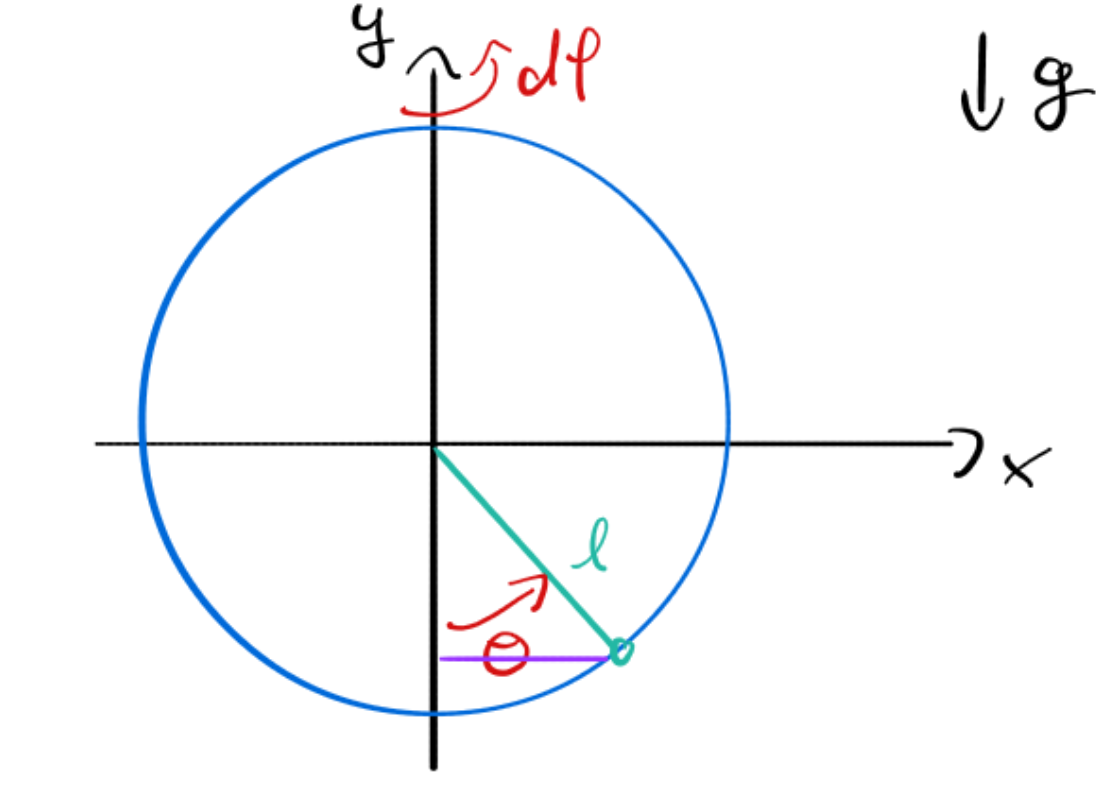
\includegraphics[width=0.6\textwidth]{images/pendoloInRotazione.png}
        \caption{Rappresentazione pendolo in rotazione}
    \end{figure}

    \begin{equation*}
        \dd{s}^2 = \ell^2 \dd{\theta}^2 + \ell^2 \sin^2\theta \, \omega^2 \dd{t}^2
        \implies K = \frac{1}{2}m \left( \ell^2 \dot{\theta}^2 + \ell^2 \sin^2\theta \, \omega^2 \right)
        \qquad U = mg(-\ell\cos\theta)
    \end{equation*}
    \begin{equation}
        \mathcal{L} = \frac{1}{2} m \ell^2 \dot{\theta}^2 + \frac{1}{2} m \ell^2 \sin^2\theta \, \omega^2 + mg\ell\cos\theta
    \end{equation}

    $\mathcal{L}$ non dipende esplicitamente dal tempo, perciò si conserva:
    \begin{equation}
        H = \pdv{\mathcal{L}}{\dot{q}}\dot{q}-\mathcal{L} =K_2-K_0+U
    \end{equation}
    \begin{equation*}
        H = m\ell^2 \dot{\theta} \cdot \dot{\theta} - \frac{m\ell^2}{2} \dot{\theta}^2 - \frac{m\ell^2}{2} \sin^2\theta \, \omega^2 - mg\ell \cos\theta
        = \frac{m\ell^2}{2} \dot{\theta}^2 - mg\ell \cos\theta - \frac{m\ell^2}{2} \omega^2 \sin^2\theta
    \end{equation*}
    \begin{equation}
        \implies \mathcal{L} = m\ell^2 \left[ \frac{\dot{\theta}^2}{2} + \frac{\omega^2}{2} \sin^2\theta + \frac{g}{\ell} \cos\theta \right]
        := m\ell^2 \mathcal{L}' \qquad
        \omega_g := \sqrt{\frac{g}{\ell}}
    \end{equation}
    \begin{remark}
        Le equazioni di Lagrange sono lineari, posso usare $\mathcal{L}$ o $\mathcal{L}'= c\mathcal{L}$ con $c\neq0$ e avere le stesse equazioni finali.
    \end{remark}
    \begin{equation*}
        H' = \frac{\dot{\theta}^2}{2}- \frac{\omega^2}{2}\sin[2](\theta) - \omega_g^2\cos(\theta)\implies E = \frac{\dot{\theta}^2}{2}+U_e(\theta)
    \end{equation*}
    
    \paragraph{Proprietà del potenziale efficace}
    Il potenziale efficace $U_e(\theta)$ è pari: $U_e(\theta) = U_e(-\theta)$. La derivata prima è
    \[
    U_e'(\theta) = -\omega^2 \sin\theta \cos\theta + \omega_g^2 \sin\theta
    \]
    Gli zeri di $U_e'(\theta)$ sono dati da
    \[
    U_e'(\theta) = 0 \iff (\omega_g^2 - \omega^2 \cos\theta)\sin\theta = 0
    \]
    quindi per $\theta = 0, \pi$ e, se $\omega > \omega_g$, anche per $\cos\theta = \frac{\omega_g^2}{\omega^2}$, cioè esistono due soluzioni simmetriche $\theta_\pm \simeq \pm \arccos\left(\frac{\omega_g^2}{\omega^2}\right)$.

    \paragraph{Stabilità degli equilibri}
    La derivata seconda è
    \[
    U_e''(\theta) = \omega_g^2 \cos\theta - \omega^2 \cos(2\theta)
    \]
    Per $\theta = 0$: $U_e''(0) = \omega_g^2 - \omega^2$ (stabile se $\omega < \omega_g$, instabile se $\omega > \omega_g$).\\
    Per $\theta = \pi$: $U_e''(\pi) = -\omega_g^2 - \omega^2$ (sempre instabile).\\
    Per $\theta = \theta_\pm$: $U_e''(\theta_\pm) = -\frac{\omega_g^4}{\omega^2} + \omega^2$, che è positivo se $\omega > \omega_g$ (stabile).

    \paragraph{Comportamento per piccoli angoli}
    Per $\omega < \omega_g$, il comportamento è simile al pendolo classico. Per $\theta$ piccoli:
    \[
    U_e(\theta) \simeq -\omega_g^2\left(1 - \frac{\theta^2}{2} \right) - \frac{\omega^2}{2} \theta^2 + o(\theta^4)
    = \frac{\omega^2_g-\omega^2}{2}\theta^2 -\omega^2_g +o(\theta^4)
    \]

    \paragraph{Transizione di stabilità}
    Quando $\omega$ raggiunge $\omega_g$, si inverte la concavità del potenziale efficace.

    \paragraph{Tipi di moto per $\omega > \omega_g$}
    \begin{itemize}
        \item $E < U(\theta_\pm)$: nessun moto
        \item $E = U(\theta_\pm)$: due punti di equilibrio (centri)
        \item $E \in \left( U(\theta_\pm), U(0) \right)$: due moti oscillatori
        \item $E = U(0) = -\omega_g^2$: punto iperbolico, due traiettorie omoclini
        \item $E > U(0)$: comportamento come un pendolo con due moti rotatori
    \end{itemize}

    %Finire qua....

\end{example}


\begin{example}
    \textbf{Pendolo sferico}\\
    La particella si muove su un anello libero di ruotare:
    \begin{equation}
        \dd{s^2}=\ell^2\dd{\theta^2}+\ell^2\sin[2](\theta)\dd{\varphi^2}\,;\qquad 
        K = \frac{m\ell^2}{2}\left( \dot{\theta}^2+\sin[2](\theta)\dot{\varphi^2} \right)
    \end{equation}
    \begin{equation}
        \mathcal{L}= \frac{m\ell^2}{2}\left( \dot{\theta}^2+\sin[2](\theta)\dot{\varphi^2} \right)+mg\ell\cos(\theta)
    \end{equation}
    E se l'anello avesse massa? $\dd{m}= \rho\dd{s}=\rho\ell\dd{\theta'}$
    \begin{equation*}
        K_{\text{anello}} = 2 \int_0^{\pi} \frac{1}{2} \, \rho \, \ell \, \dd{\theta'} \, \ell^2 \sin^2\theta' \, \dot{\varphi}^2
        = \frac{2}{2} \, \dot{\varphi}^2 \, \ell^3 \, \rho \int_0^{\pi} \sin^2\theta' \, \dd{\theta'}
    \end{equation*}
    \begin{equation}
        = \ell^3 \dot{\varphi}^2 \rho \int_0^{\pi} \frac{1 - \cos 2\theta}{2} \, \dd{\theta}
        = \frac{\ell^3 \dot{\varphi}^2 \rho}{2} \left[ \theta - \frac{\sin 2\theta}{2} \right]_0^{\pi}
        = \frac{\ell^3 \dot{\varphi}^2 \rho}{2} \cdot \pi
    \end{equation}
    \begin{equation}
        M = \rho \cdot 2\pi\ell \implies K_\text{anello}= \frac{M \ell^2 \dot{\varphi}^2}{4}\qquad
        r = \frac{M}{2m} \qquad \omega_g = \sqrt{\frac{g}{\ell}}
    \end{equation}
    \begin{equation}
        \implies \mathcal{L}= K-U = m\ell^2\left( \frac{1}{2}\dot{\theta}^2 +\frac{1}{2}\sin[2](\theta)\dot{\varphi}^2+ \frac{r}{2}\dot{\varphi}^2+ \omega^2_g\cos(\theta)\right)
    \end{equation}
    \begin{equation}
        \pdv{\mathcal{L}}{\varphi}=0\implies P_\varphi= \frac{\mathcal{L}'}{\dot{\varphi}}= \left( \sin[2](\theta)+r \right)\dot{\varphi}\equiv c \text{ costante}
    \end{equation}

    Il segno di $c $ è quello di $\dot{\varphi}(0)$. Studiamo $c>0$:
    \begin{equation}
        \dot{\varphi}(t)=\frac{c}{\sin[2](\theta(t))+r}>0 \quad \forall\;t
    \end{equation}
    \begin{equation*}
        \pdv{\mathcal{L}'}{t} = 0 \implies H' = K' + U' = \frac{\dot{\theta}^2}{2} + \frac{\sin^2\theta}{2} \dot{\varphi}^2 + \frac{r}{2} \dot{\varphi}^2 - \omega_g^2 \cos\theta
    \end{equation*}
    \begin{equation*}
        = \frac{\dot{\theta}^2}{2} + \frac{\sin^2\theta}{2} \cdot \frac{c^2}{(\sin^2\theta + r)^2} + \frac{r}{2} \cdot \frac{c^2}{(\sin^2\theta + r)^2} - \omega_g^2 \cos\theta
    \end{equation*}
    \begin{equation}
        = \frac{\dot{\theta}^2}{2} + \frac{c^2}{2(\sin^2\theta + r)} - \omega_g^2 \cos\theta = E := \frac{\dot{\theta}^2}{2} + U_e(\theta)
    \end{equation}

    Studiamo ora le orbite del sistema:
    \begin{equation}
        U_e(\theta) = \frac{1}{2} \cdot \frac{c^2}{\sin^2\theta + r} - \omega_g^2 \cos\theta \implies 
        U_e(\theta) = U_e(-\theta)
    \end{equation}
    \begin{equation}
        U_e'(\theta) = \omega_g^2 \sin\theta - \frac{c^2}{(\sin^2\theta + r)^2} \cdot 2\sin\theta \cos\theta
    \end{equation}
    \begin{equation}
        \implies U_e' = 0 \iff \theta = 0, \pi \text{ e le soluzioni di }
        (\sin^2\theta + r)^2 = \frac{c^2}{\omega_g^2 \cos\theta}
    \end{equation}
    \begin{equation}
        \text{se } r^2 < \frac{c^2}{\omega_g^2} \quad \exists \text{ sol. } \theta_+(r) \in \left[ 0, \frac{\pi}{2} \right], \quad \theta_-(r) = -\theta_+(r) \in \left[ -\frac{\pi}{2}, 0 \right]
    \end{equation}

    Per $r> \frac{c}{\omega_g}$ non esistono soluzioni. Consideriamo prima questo caso:
    \begin{equation}
        r > \frac{c}{\omega_g} \qquad 
        U_e' = \left[ \dots \right] \sin\theta \,, \quad \text{con } \left[ \dots \right] > 0 
    \end{equation}
    \begin{equation}
        \implies U_e'(\theta) > 0 \quad \text{in } (0,\pi) \,;\qquad 
        U_e(0) = \frac{c^2}{2r} - \omega_g^2 \,, \quad 
        U_e(\pi) = \frac{c^2}{2r} + \omega_g^2
    \end{equation}

    Ci ricaviamo quindi le forme dell'orbita a seconda dell'energia:
    \begin{itemize}
        \item $E = \frac{c^2}{2r} - \omega_g^2 =: E_{\min}$: equilibrio
        \item $E \in (E_{\min}, E_{\max})$: moti oscillatori
        \item $E = \frac{c^2}{2r} + \omega_g^2 =: E_{\max}$: connessioni eterocline
        \item $E > E_{\max}$: 2 moti non limitati in $\theta$
    \end{itemize}

    Invece per $r<\frac{c}{\omega_g}$:
    \begin{equation}
        U_e'(\theta) = \left[ \dots \right] \sin\theta, \quad \text{con } \left[ \dots \right] < 0 \text{ per } \theta \in [0, \theta_+]
    \end{equation}
    \begin{equation}
        \Rightarrow U_e'(\theta) < 0 \quad \text{per } \theta \in (0, \theta_+)
    \end{equation}

    Da cui possiamo ricavare le orbite:
    \begin{itemize}
        \item $E = E_{\min}$: 2 equilibri
        In questo caso c'è $\theta$ costante e $\dot{\varphi}$ costante $\implies$, cioè la massa è in moto circolare uniforme.
        
        \item $E \in (E_{\min}, U_e(0))$: 2 moti circolari

        \item $E = U_e(0)$: 2 omoclini con equilibrio iperbolico

        \item $E \in (U_e(0), E_{\max})$: 1 moto periodico
        
        \item $\sim$ poi come prima.
    \end{itemize}
     %bdhbhsbfs

\end{example}

\begin{example}
    \textbf{Particella su superficie di rotazione}\\
    Abbiamo una curva $x(z)$, $x(z) > 0 \quad \forall z \in \mathbb{R} \quad \max x(z) = x(0) \quad x(z) = x(-z) $\\ 
    $ x(z) \xrightarrow{|z|\to \infty} 0$ per cui consideriamo la superficie in basi cilindriche:
    \begin{equation*}
        \begin{pmatrix}
            r\cos\varphi\\
            r\sin\varphi\\
            z
        \end{pmatrix}
        =
        \begin{pmatrix}
            x\\y\\z
        \end{pmatrix}
        \qquad r = f(z) = x(z)
    \end{equation*}
    \begin{equation*}
        \mathcal{L} = K = \frac{m}{2} \left( \dot{r}^2 + r^2 \dot{\varphi}^2 + \dot{z}^2 \right)\bigg|_{r = f(z)} =
        \frac{m}{2} \left( f'(z)^2 \dot{z}^2 + f(z)^2 \dot{\varphi}^2 + \dot{z}^2 \right)
    \end{equation*}
    \begin{equation}
        = \frac{m}{2} \left( \left(1 + f'(z)^2 \right) \dot{z}^2 + f(z)^2 \dot{\varphi}^2 \right)
    \end{equation}
    \begin{equation}
        \implies H = K = E \;;\quad \varphi \text{ ciclica} \implies p_\varphi = \pdv{\mathcal{L}}{\dot{\varphi}} = mf(z)^2 \dot{\varphi} = c 
        \implies \dot{\varphi} = \frac{c}{m f(z)^2}
    \end{equation}
    \begin{equation}
        \implies E = \frac{m}{2} \left( 1 + f'(z)^2 \right) \dot{z}^2 + \frac{c^2}{2m f(z)^2}
    \end{equation}

    %jdknsfjksnvs

\end{example}


\subsection{Formulazione variazionale}
\begin{example}
    Qual è la curva di lunghezza minima tra due punti nel piano? Ovviamente sappiamo che la risposta è il segmento.
\end{example}
Consideriamo le funzioni $x\mapsto y= f(x):[x_2,x_2]\mapsto \mathbb{R}$ t.c. $f(x_1)=y_1, \,f(x_2)=x_2$.\\
La lunghezza dell'arco di funzione:
\begin{equation}
    \ell[f]=\int_{x_1}^{x_2}\sqrt{1+(f'(x))^2}\dd{x}            
\end{equation}
dove $\ell: \Gamma\rightarrow \mathbb{R}$ è un \textit{funzionale} e $f\in\Gamma$ è la classe di funzioni.\\
Più in generale se consideriamo uno spazio di funzioni:
\begin{equation}
    \Gamma= \left\{ f: x\mapsto y , f\in \mathcal{C}^2, f(x_1)=y_1, f(x_2)= y_2 \right\}
\end{equation}
possiamo definire un funzionale:
\begin{equation}
    F[f ]:= \int_{x_1}^{x_2}\mathcal{F}(f(x),f'(x),x)\dd{x}
\end{equation}
dove $\mathcal{F}:\mathbb{R}^3\rightarrow \mathbb{R}$ è detta \textit{densità del funzionale}, supponiamo $\mathcal{F}\in \mathcal{C}^2$.

\begin{remark}
    Ricordiamo la definizione di \textit{differenziale primo} di $g: \mathbb{R}^n \rightarrow \mathbb{R}$:
    \begin{equation}
        \dd{g}\eval_{x}(h) =\nabla g(x)\cdot h = \lim_{\varepsilon \to 0} \frac{g(x + \varepsilon h) - g(x)}{\varepsilon} 
        = \dv{\varepsilon} g(x + \varepsilon h)\bigg|_{\varepsilon = 0}
    \end{equation}
\end{remark}

\begin{definition}
    Si chiama \textit{differenziale debole} o di Gateaux o \textit{variazione di Lagrange} del funzionale $F $ la quantità:
    \begin{equation}
        \delta F = \lim_{\varepsilon\to 0}\frac{F[f+\varepsilon\delta f]-F[f]}{\varepsilon}= \dv{\varepsilon} F[f+\varepsilon\delta f ]\eval_{\varepsilon=0}
    \end{equation}
    dove gli incrementi $\delta f $ sono definiti tali che $\delta f(x_1)= \delta f(x_2)=0$
\end{definition}

\begin{equation}
    F\left[ f + \varepsilon \, \delta f \right] 
    = \int_{x_1}^{x_2} \mathcal{F}\left( f(x) + \varepsilon \, \delta f(x), f'(x) + \varepsilon \, \delta f'(x), x \right) \dd{x}
\end{equation}
\begin{equation*}
    = \int_{x_1}^{x_2} \mathcal{F}(f, f', x) \dd{x} 
    + \varepsilon \int_{x_1}^{x_2} \left( \pdv{\mathcal{F}}{f} \delta f + \pdv{\mathcal{F}}{f'} \delta f' \right) \dd{x}
\end{equation*}
\begin{equation}
    + \frac{\varepsilon^2}{2} \int_{x_1}^{x_2} \left( 
    \pdv[2]{\mathcal{F}}{f} \, \delta f^2 
    + 2 \pdv{\mathcal{F}}{f}{f'} \, \delta f \, \delta f' 
    + \pdv[2]{\mathcal{F}}{{f'}} \, \delta f'^2 
    \right) \dd{x} + o(\varepsilon^2)
\end{equation}
\begin{equation}
    \implies \delta F = \int_{x_1}^{x_2} \left( \pdv{\mathcal{F}}{f} \, \delta f + \pdv{\mathcal{F}}{f'} \, \delta f' \right) \dd{x} 
    = \int_{x_1}^{x_2} \left[ \pdv{\mathcal{F}}{f} - \dv{x} \left( \pdv{\mathcal{F}}{f'} \right) \right] \delta f \, \dd{x}
\end{equation}

\begin{remark}
    \begin{equation*}
    \delta F = \dd{F}[f](\delta f)
    \end{equation*}    
\end{remark}

Ora cerchiamo i punti critici di $F$; cioè le $f$ t.c. $\delta F = 0 \quad \forall \, \delta f$

\begin{proposition}
    \begin{equation}
        \delta F = 0 \quad \forall\,\delta f \iff \begin{cases}
            \pdv{\mathcal{F}}{f} - \dv{x} \pdv{\mathcal{F}}{f'}=0 \\
            f(x_1)=y_1 \quad f(x_2)= y_2
        \end{cases}
    \end{equation}
\end{proposition}
In cui riconosciamo le equazioni di Eulero-Lagrange

Si dimostra utilizzando il \textit{lemma fondamentale del calcolo delle variazioni}:
\begin{lemma}
    Se $\alpha(x)$ è una funzione continua su $[x_1,x_2]$, allora:
    \begin{equation}
        \int_{x_1}^{x_2} \alpha(x)\delta f \dd{x}= 0 \quad \forall\,\delta f  \iff \alpha(x)=0
    \end{equation}
\end{lemma}
\begin{proof}
    $\impliedby$ è immediata.\\
    $\implies$ Supponiamo che $\int_{x_1}^{x_2} \alpha(x)\delta f \dd{x}= 0 \quad \forall\,\delta f$ 
    e che $\exists\,\bar{x}$ t.c. $\alpha(\bar{x})>0$ per continuità allora $\exists\,I_{\bar{x}}\subseteq[x_1,x_2]$ t.c. $\alpha(x)>0, \forall\,x\in I_{\bar{x}}$.\\
    Scelgo poi un $\hat{\delta f}$ t.c $\hat{\delta f}(x)>0 \;\forall\,x\in I_{\bar{x}}$ e $\hat{\delta f}(x)\equiv 0 \;\forall\,x \notin I_{\bar{x}} $:
    \begin{equation*}
        \int_{x_1}^{x_2}\alpha(x)\hat{\delta f}(x)\dd{x}= \int_{I_{\bar{x}}} \alpha(x)\hat{\delta f}(x)\dd{x}>0 \quad\text{ Assurdo!}
    \end{equation*}
\end{proof}


\begin{remark}
Il problema è leggermente diverso dal classico problema di Cauchy;
 ci sono conseguenze nell'avere condizioni al contorno al posto di iniziali.
\end{remark}

\begin{remark}
    \begin{equation*}
        \pdv{\mathcal{F}}{f} - \dv{x} \pdv{\mathcal{F}}{f'} 
        = \pdv{\mathcal{F}}{f} - \pdv[2]{\mathcal{F}}{f'}{f} f' 
        - \pdv[2]{\mathcal{F}}{{f'}} f'' 
        - \pdv[2]{\mathcal{F}}{x}{f'} = 0  
    \end{equation*}
    Si può scrivere come \( f''(x) = G(f(x), f'(x), x) \) solo se \( \pdv[2]{\mathcal{F}}{{f'}}\neq 0 \).
\end{remark}

\begin{equation*}
    \Delta \tilde{F} = F\left[ \tilde{f} + \varepsilon \, \delta f \right] - F[\tilde{f}]   
\end{equation*}
\begin{equation*}
    = \frac{\varepsilon^2}{2} \int_{x_1}^{x_2} \left\{
    \pdv[2]{\mathcal{F}}{f}\eval_{\tilde{f}} (\delta f)^2 
    + 2 \pdv[2]{\mathcal{F}}{f}{{f'}}\eval_{\tilde{f}} \dv{x}(\delta f)^2 
    + \pdv[2]{\mathcal{F}}{{f'}}\eval_{\tilde{f}} (\delta f')^2 
    \right\} \dd{x} + o(\varepsilon^2)
\end{equation*}
\begin{equation*}
    = \frac{\varepsilon^2}{2} \int_{x_1}^{x_2} \left[
    \left( \pdv[2]{\mathcal{F}}{f} \eval_{\tilde{f}}
    - \dv{x} \left( \pdv[2]{\mathcal{F}}{f}{{f'}} \right)\eval_{\tilde{f}}
    \right) \delta f^2+
    \pdv[2]{\mathcal{F}}{{f'}}\eval_{\tilde{f}} (\delta f')^2 \right] \dd{x}
    + \eval{\pdv[2]{\mathcal{F}}{{f'}} \, \delta f^2}_{x_1}^{x_2}
    + o(\varepsilon^2)
\end{equation*}
\begin{equation*}
    = \frac{\varepsilon^2}{2} \int_{x_1}^{x_2}
    \left[ Q(x) \, \delta f^2(x)+ P(x) \, \delta f'^2(x) \right] \dd{x} + o(\varepsilon^2)
\end{equation*}

Se $\int_{x_1}^{x_2} Q\, \delta f^2 + P\, \delta f'^2\, \dd{x} > 0 $ per $\varepsilon$ abbastanza piccolo,
allora vale:
\begin{equation*}
\Delta \tilde{F} = F\left[ \tilde{f} + \varepsilon \delta f \right] - F[\tilde{f}] > 0
\implies \tilde{f} \text{ minimo (e viceversa per i massimi)}
\end{equation*}
